
\clearpage

\hspace*{-1cm} \vspace*{-0.2cm}
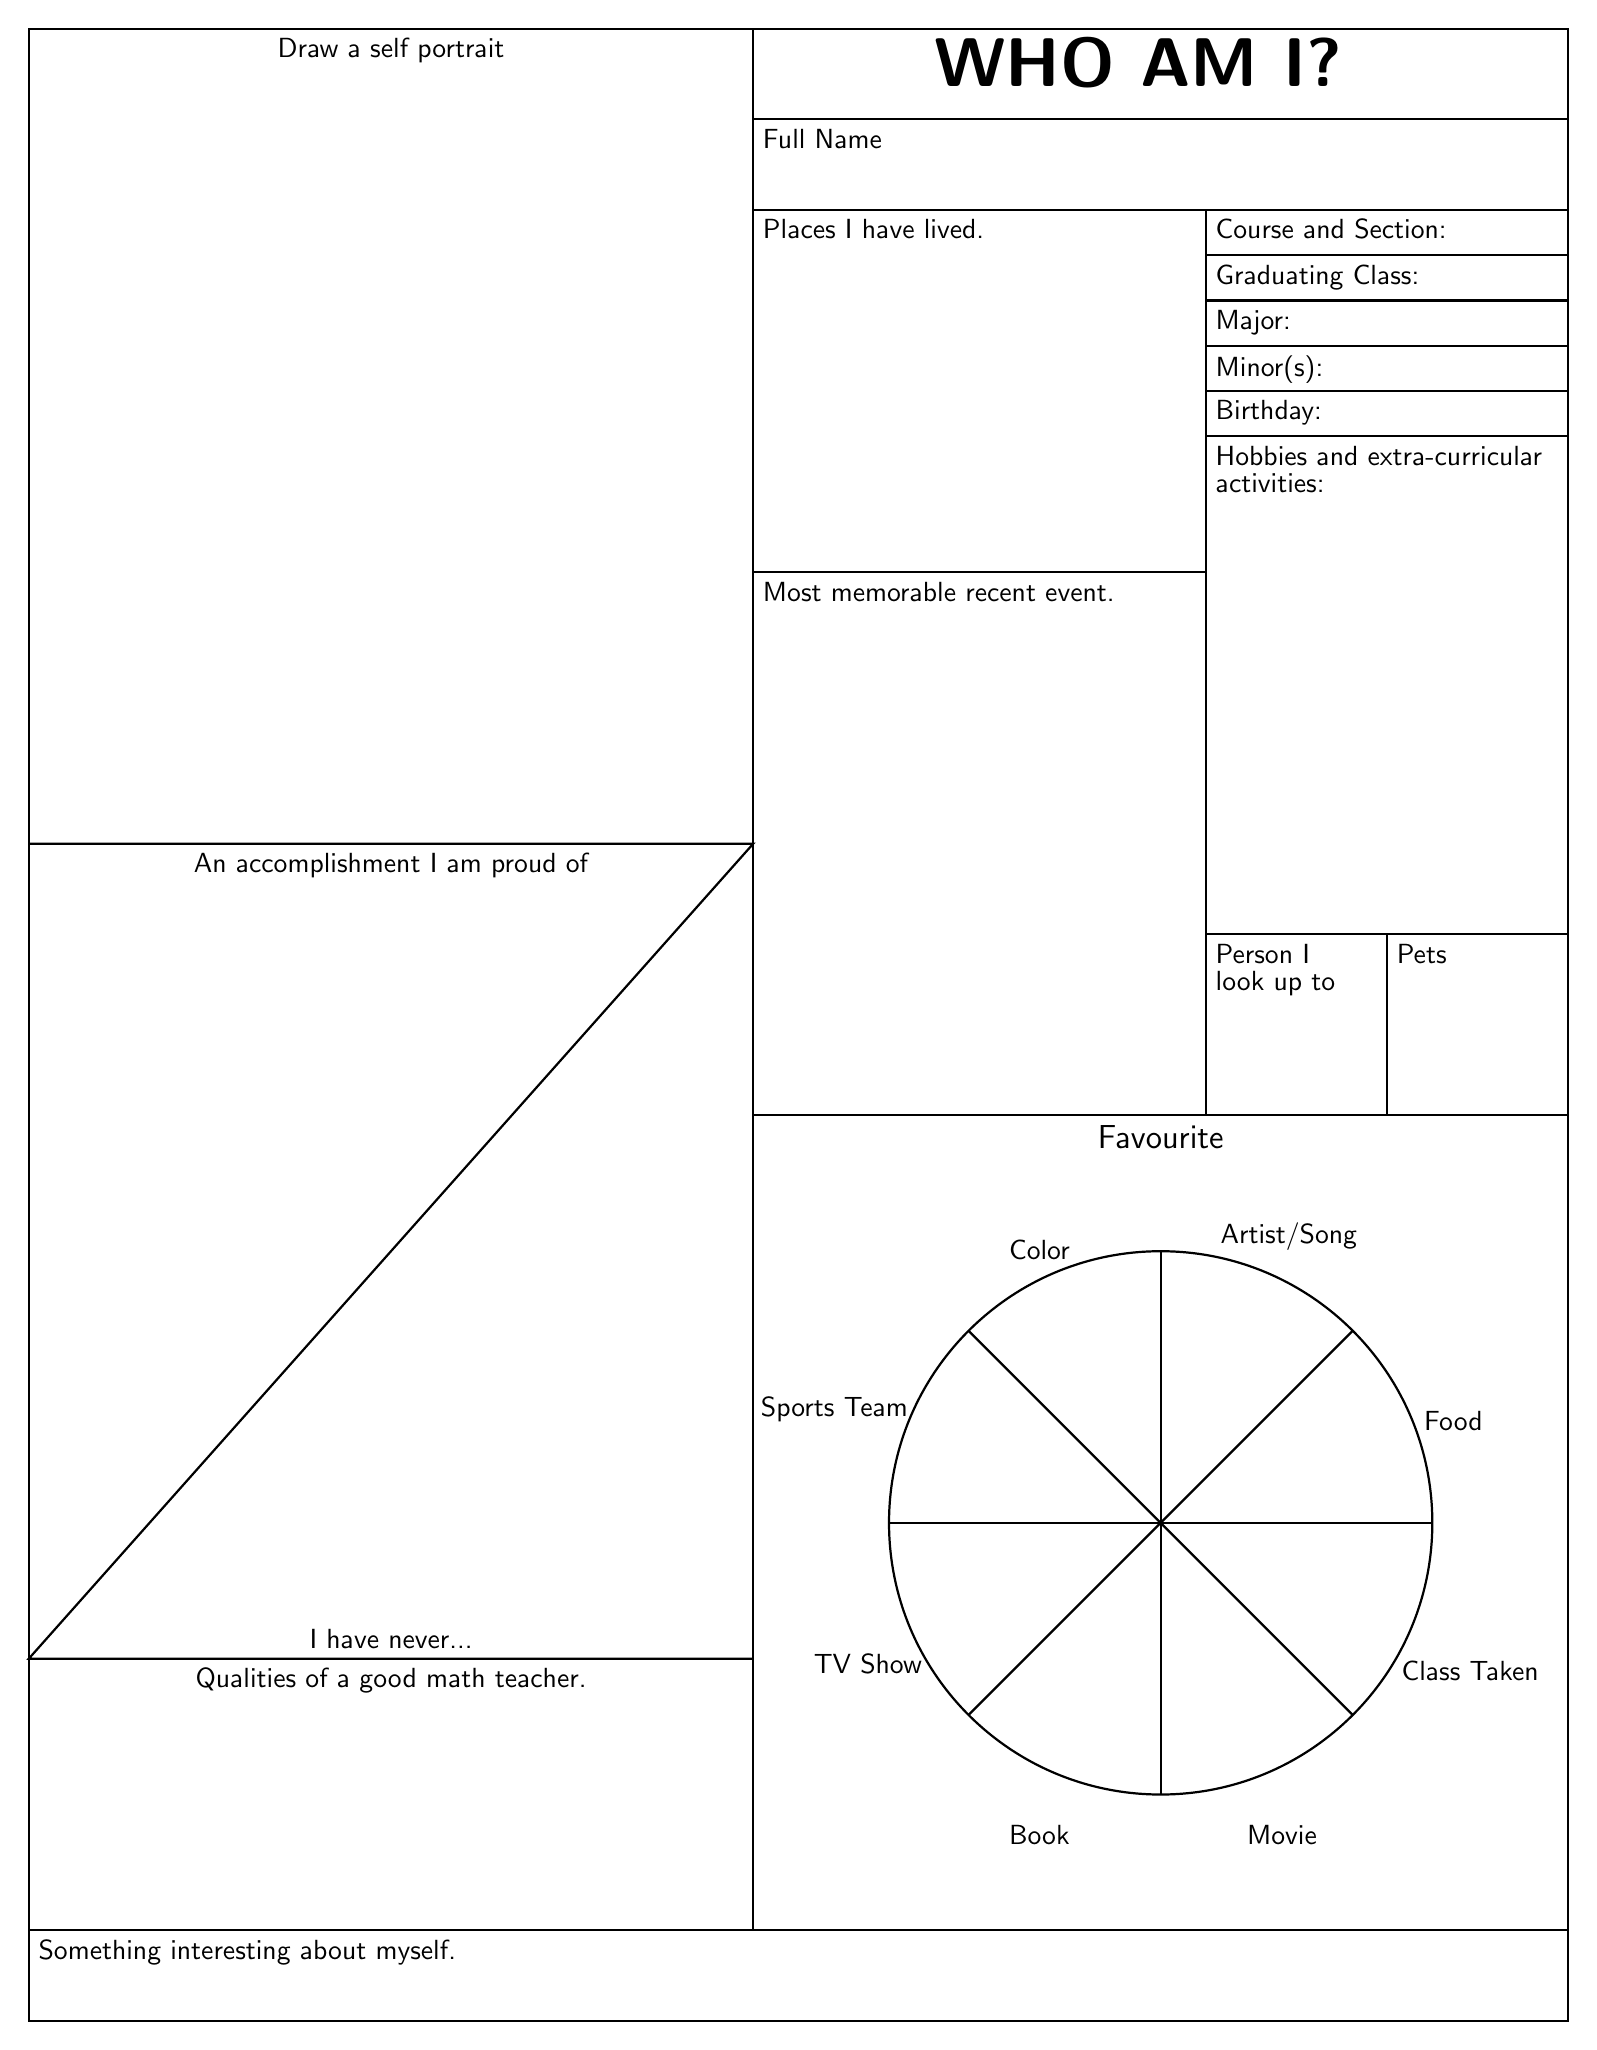
\begin{tikzpicture}[y=2.3cm, x=2.3cm,font=\sffamily]

  % Outline around the whole thing.
  \draw[thick,black] (0,0.5) -- (8.5,0.5) -- (8.5,11) -- (0,11) -- cycle;
  \draw[thick,black] (0,0.5) -- (0,0) -- (8.5,0) -- (8.5,0.5);
  \draw[thick,black] (0,0.5) -- (8.5,0.5);

  % Boxes for the left side.
  \draw[thick,black] (4,0.5) -- (4,11);
  \draw[thick,black] (0,6.5) -- (4,6.5) -- (0,2) -- (4,2);

  % Boxes for the right side.
  \draw[thick,black] (4,10.5) -- (8.5,10.5);
  \draw[thick,black] (4,10) -- (8.5,10);
  \draw[thick,black] (6.5,5) -- (6.5,10);
  \draw[thick,black] (4,5) -- (8.5,5);

  % boxes in the upper right
  \draw[thick,black] (4,8) -- (6.5,8);
  \draw[thick,black] (6.5,9.75) -- (8.5,9.75);
  \draw[thick,black] (6.5,9.5) -- (8.5,9.5);
  \draw[thick,black] (6.5,9.25) -- (8.5,9.25);
  \draw[thick,black] (6.5,9.0) -- (8.5,9.0);
  \draw[thick,black] (6.5,8.75) -- (8.5,8.75);

  \draw[thick,black] (6.5,6) -- (8.5,6);
  \draw[thick,black] (7.5,6) -- (7.5,5);

  % Text on the left side
  \node[black,anchor=north] at (2,11) {Draw a self portrait};
  \node[black,anchor=north] at (2,6.5) {An accomplishment I am proud of};
  \node[black,anchor=south] at (2,2) {I have never...};
  \node[black,anchor=north] at (2,2) {Qualities of a good math teacher.};
  \node[black,anchor=north west] at (0,0.5) {Something interesting about myself.};

  % Text on the upper right
  \node[black,anchor=north] at (6.125,11) {\Huge \textbf{WHO AM I?}};
  \node[black,anchor=north west] at (4,10.5) {Full Name};
  \node[black,anchor=north west] at (4,10) {Places I have lived.};
  \node[black,anchor=north west] at (4,8) {Most memorable recent event.};
  
  \node[black,anchor=north west] at (6.5,10) {Course and Section:};
  \node[black,anchor=north west] at (6.5,9.75) {Graduating Class:};
  \node[black,anchor=north west] at (6.5,9.50) {Major:};
  \node[black,anchor=north west] at (6.5,9.25) {Minor(s):};
  \node[black,anchor=north west] at (6.5,9.00) {Birthday:};
  \node[black,anchor=north west] at (6.5,8.75) {Hobbies and extra-curricular};
  \node[black,anchor=north west] at (6.5,8.60) {activities:};
  \node[black,anchor=north west] at (6.5,6) {Person I};
  \node[black,anchor=north west] at (6.5,5.85) {look up to};
  \node[black,anchor=north west] at (7.5,6) {Pets};
  \node[black,anchor=north] at (6.25,5) {\large Favourite};
  
  % Draw the pie chart
  \begin{scope}[shift={(6.25,2.75)}]
    \draw[thick,black] (0,0) circle (1.5);
    \draw[thick,black] (0:1.5)   -- (180:1.5);
    \draw[thick,black] (45:1.5)  -- (225:1.5);
    \draw[thick,black] (90:1.5)  -- (270:1.5);
    \draw[thick,black] (135:1.5) -- (315:1.5);

    \node[black,anchor=north] at ( 22.5:1.75) {Food};
    \node[black,anchor=north] at ( 67.5:1.85) {Artist/Song};
    \node[black,anchor=north] at (112.5:1.75) {Color};
    \node[black,anchor=north] at (157.5:1.95) {Sports Team};
    \node[black,anchor=north] at (202.5:1.75) {TV Show};
    \node[black,anchor=north] at (247.5:1.75) {Book};
    \node[black,anchor=north] at (292.5:1.75) {Movie};
    \node[black,anchor=north] at (337.5:1.85) {Class Taken};


  \end{scope}
  
\end{tikzpicture}

\clearpage

%%% Local Variables:
%%% mode: latex
%%% TeX-master: "linearAlgebraWorkbook"
%%% End:
